%%%%%%%%%%%%%%%%%%%%%%%%%%%%%%%%%
%
%       EXERCÍCIO
%
%%%%%%%%%%%%%%%%%%%%%%%%%%%%%%%%%

\definevalorquestao

\begin{exercicioBanco}[\valorquestao]
Considere a função afim cujo gráfico está desenhado abaixo.
%

%
\begin{center}
    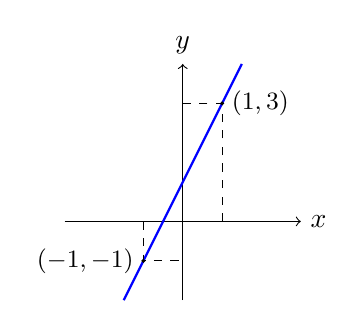
\begin{tikzpicture}[scale=0.5]
        % Eixos
        \draw[->] (-3,0) -- (3,0) node[right] {\(x\)};
        \draw[->] (0,-2) -- (0,4) node[above] {\(y\)};
              
        % Gráfico
        \draw[domain=-1.5:1.5, smooth, variable=\x, blue, thick] 
        plot ({\x}, {2*\x + 1});
              
        % Pontos escolhidos
        \draw[dashed] (-1,0) -- (-1,-1) -- (0,-1);
        \draw[dashed] (1,0) -- (1,3) -- (0,3);
             
        % Marcando os pontos
        \filldraw (-1,-1) circle (1pt) node[left] {\small\((-1,-1)\)};
        \filldraw (1,3) circle (1pt) node[right] {\small\((1,3)\)};
    \end{tikzpicture}
\end{center}
%
Determine o zero dessa função.

% Define as alternativas
\newcommand{\alternativas}{%
    \begin{center}
        \begin{tabularx}{\textwidth}{XXXXX}
            (a) \(-\dfrac{1}{3}\). &
            (b) \(-\dfrac{2}{3}\). &
            (c) \(-\dfrac{1}{2}\). &
            (d) \(\dfrac{1}{4}\). &
            (e) \(\dfrac{3}{4}\).
        \end{tabularx}
    \end{center}
}

% Define a resposta correta
\newcommand{\resposta}{C}

% Lógica condicional para exibição
\ifdefstring{\atividade}{lista}{%
    \alternativas
    \vspace{0.5em}
    
    \noindent\textbf{Resposta:} letra \textbf{\resposta}.
}{%
    \ifdefstring{\modo}{objetivo}{%
        \alternativas
    }{%
        % modo = discursiva → não mostra alternativas
    }
}
\end{exercicioBanco}

